\documentclass[10pt]{beamer}
\usetheme{metropolis}
\usepackage{booktabs}
\usepackage{tabularx}
\usepackage{calc}
\usepackage{tikz}
%\usepackage[sfdefault]{FiraSans}
%\usepackage[scaled]{FiraMono}
\usetikzlibrary{shapes.geometric, arrows, positioning, decorations.pathreplacing}

% Setup for faculty images
\newlength{\imageheight}
\setlength{\imageheight}{3.5cm}

% Define CSUF brand colors
\definecolor{titanblue}{HTML}{00244E}
\definecolor{mediumblue}{HTML}{0F3F8C}
\definecolor{skyblue}{HTML}{EBFBFF}
\definecolor{titanorange}{HTML}{FF7900}
\definecolor{titangray}{HTML}{F5F5F5}
\definecolor{titantext}{HTML}{222222}

% Customize metropolis theme colors
\setbeamercolor{normal text}{fg=titantext, bg=white}
\setbeamercolor{alerted text}{fg=titanorange}
\setbeamercolor{example text}{fg=mediumblue}

% Title page colors
\setbeamercolor{title}{fg=titanblue, bg=white}
\setbeamercolor{subtitle}{fg=mediumblue, bg=white}
\setbeamercolor{institute}{fg=titanorange, bg=white}
\setbeamercolor{date}{fg=titanblue, bg=white}

% Frame title colors
\setbeamercolor{frametitle}{fg=white, bg=titanblue}
\setbeamercolor{framesubtitle}{fg=mediumblue, bg=white}

% Block environment colors
\setbeamercolor{block title}{fg=white, bg=titanblue}
\setbeamercolor{block body}{fg=titantext, bg=skyblue!10}

% Item colors
\setbeamercolor{itemize item}{fg=titanorange}
\setbeamercolor{itemize subitem}{fg=mediumblue}
\setbeamercolor{itemize subsubitem}{fg=titanblue}

% Footer and header colors
\setbeamercolor{footer}{fg=titantext}
\setbeamercolor{header}{fg=titanblue}

% Custom TikZ embellishments for POSC 315 Beamer slides
\usepackage{tikz}
\usetikzlibrary{shadows,arrows.meta,positioning,shapes.multipart}

% Boxed text for emphasis
\newcommand{\tikzbox}[2][]{
  \begin{tikzpicture}
    \node[draw=mediumblue, fill=skyblue!20, thick, rounded corners, inner sep=10pt, text width=0.9\textwidth,#1] {#2};
  \end{tikzpicture}
}

% Horizontal divider with arrow
\newcommand{\tikzdivider}{
  \begin{center}
  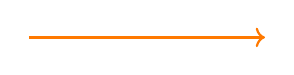
\begin{tikzpicture}
    \draw[->, thick, titanorange] (0,0) -- (3,0);
  \end{tikzpicture}
  \end{center}
}

% Highlighted comparison row (e.g., for causation slides)
\newcommand{\relationrow}[2]{
  \begin{tikzpicture}
    \node[draw=none, fill=titangray!50, rounded corners, text width=0.9\textwidth, inner sep=8pt] {
      \textbf{#1} \hfill #2
    };
  \end{tikzpicture}
}

% Framed callout block
\newcommand{\callout}[1]{
  \begin{tikzpicture}
    \node[draw=titanorange, fill=white, thick, rounded corners, inner sep=10pt, text width=0.9\textwidth] {
      \textit{#1}
    };
  \end{tikzpicture}
}

% Customize fonts
\setbeamerfont{title}{size=\Large, series=\bfseries}
\setbeamerfont{frametitle}{size=\large, series=\bfseries}

% Simple title page template
\defbeamertemplate*{title page}{customized}[1][]
{
\vspace{1cm}
 {\usebeamerfont{title}\usebeamercolor[fg]{title}\inserttitle\par}
\vspace{0.5cm}
 {\usebeamerfont{subtitle}\usebeamercolor[fg]{subtitle}\insertsubtitle\par}
\vspace{0.5cm}
 {\usebeamerfont{date}\usebeamercolor[fg]{date}\insertdate\par}
\vfill
 {\insertinstitute\par}
}

% Add progress bar
\makeatletter
\setbeamertemplate{headline}{%
\begin{beamercolorbox}[wd=\paperwidth,ht=0.4cm,dp=0cm]{titanblue}%
\begin{tikzpicture}
\pgfmathsetmacro{\progress}{\insertframenumber/\inserttotalframenumber}
\fill[titanorange] (0,0) rectangle (\progress*\paperwidth,0.4cm);
\end{tikzpicture}%
\end{beamercolorbox}%
}
\makeatother

\begin{document}

\title{Understanding Politics and Public Policy}
\subtitle{Foundations and Core Concepts\\POSC 315: Introduction to Public Policy\\Lecture 9-1: Policy Analysis Part 1}
\date{David P. Adams, Ph.D.}
\institute{California State University, Fullerton}

\maketitle


\begin{frame}{Overview}

\begin{block}{}
    \begin{itemize}
        \item General Concepts of Policy Analysis
        \item Outputs vs. Outcomes
        \item Role of Policy Analysis in the Policy Process
        \item Understanding Causation
        \item Brief History of Policy Analysis
        \item Role of the Policy Analyst
        \item Modern Approaches
        \item Applied Policy Analysis: Let's Try It!
    \end{itemize}
\end{block}

\end{frame}


\begin{frame}{General Concepts of Policy Analysis}

\tikzbox{
    \textbf{What is Policy Analysis?} \\
    A systematic approach to evaluating policy alternatives for addressing public problems using data and reasoned arguments.

    \vspace{0.8em}
    \textbf{Core Purpose:} Provide clear, objective information to decision-makers.

    \vspace{0.8em}
    \textbf{Key Question:} How can we use evidence to determine which policies are most effective?
}

\end{frame}


\begin{frame}{Outputs vs. Outcomes}

\tikzbox{
    \textbf{Outputs:}
    \begin{itemize}
        \item Measurable things an agency produces
        \item Tangible efforts, easy to track
        \item Examples: traffic signals, people served, laws passed
    \end{itemize}

    \textbf{Outcomes:}
    \begin{itemize}
        \item Actual effects on society
        \item Harder to quantify
        \item Examples: accident reduction, improved health
    \end{itemize}

    \vspace{0.4em}
    \textbf{Distinction:} Outputs show what was done; outcomes show what difference it made.
}

\end{frame}


\begin{frame}{Understanding Causation}

\tikzbox{
    \textbf{Causation} = Relationship between cause and effect

    \vspace{0.5em}
    \textbf{To establish causation:}
    \begin{itemize}
        \item Temporal sequence (cause precedes effect)
        \item Correlation
        \item No spuriousness (other factors ruled out)
    \end{itemize}
}

\end{frame}


\begin{frame}{Understanding Causation (continued)}

\relationrow{Positive}{Education ↑ → Income ↑}

\tikzdivider

\relationrow{Negative}{Cigarette Tax ↑ → Smoking ↓}

\tikzdivider

\relationrow{No Relationship}{Ice Cream Sales $\nrightarrow$ Crime Rate}

\end{frame}


\begin{frame}{History of Policy Analysis}

\tikzbox{
    \textbf{Early Developments:}
    \begin{itemize}
        \item 1908: \textit{Muller v. Oregon} — Brandeis Brief
        \item Rise of social science in governance
        \item New Deal → growth of policy advisors
        \item WWII → operations research techniques
    \end{itemize}
}

\end{frame}


\begin{frame}{Lasswell’s Policy Science}

\tikzbox{
    \textbf{Lasswell's Principles:}
    \begin{itemize}
        \item Problem-solving orientation
        \item Multidisciplinary
        \item Acknowledges values in policy decisions
    \end{itemize}

    \vspace{0.5em}
    \callout{``In a democracy, values matter as much as facts.''}
}

\end{frame}


\begin{frame}{A Policy Science}

\tikzbox{
    \textbf{Key Traits:}
    \begin{itemize}
        \item Applied & practical
        \item Interdisciplinary
        \item Empirical & theoretical
        \item Aims to improve public decisions
    \end{itemize}
}

\end{frame}


\begin{frame}{Growth and Evolution}

\tikzbox{
    \begin{itemize}
        \item Great Society → demand for analysts
        \item Dominance of economic rationality
        \item Rise of modeling & forecasting
        \item Limits of technical approaches become visible
    \end{itemize}
}

\end{frame}

\end{document}
